\documentclass{article}
\usepackage[utf8]{inputenc}
\usepackage[spanish,es-nodecimaldot,es-tabla]{babel}
\usepackage{amsmath}
\usepackage{graphicx}
\usepackage[colorlinks=true, allcolors=blue]{hyperref}
\usepackage[makeroom]{cancel}
% hyperref -->autoref, amsmath -->split
\usepackage{subfig,placeins}
\usepackage{libertine}
\usepackage[libertine]{newtxmath}
\graphicspath{{./figs/}{./imgs/}}
\usepackage[font=small,labelfont=bf]{caption}
\usepackage{listings,figs/tuneatantito}
\newcommand\pder[2]{\ensuremath
{\dfrac{\partial#1}{\partial#2}}} 
\newcommand{\ppder}[2]{ \ensuremath {\dfrac{\partial^2
#1}{\partial #2^2}}}
\newcommand{\ppcder}[3]{ \ensuremath {\dfrac{\partial^2
#1}{\partial #2\partial #3}}}
\numberwithin{figure}{section}
\numberwithin{equation}{section} %enumerar ecuacion 
															%por seccion

\title{Tarea 4}
\author{
\href{https://pedraza-espitia.github.io/modnum/}
{Pedraza-Espitia S.}}
\date{}

\begin{document}

\maketitle

\section{Circulación atmosférica y circulación oceánica}
Componentes de los modelos son las condiciones iniciales (en el tiempo), las condiciones de frontera (en el espacio),  eso nos permite modelar cada parcela, como se muestra en la \autoref{fig:esquemacompomod}.
Las condiciones de frontera pueden indicar valores fijos, y variaciones de propiedades (como intercambios de energía o momento).
También se pueden agregar términos que indiquen fuentes, sumideros, amortiguamientos, forzamientos, etc.

\begin{figure}[htp]
\centering
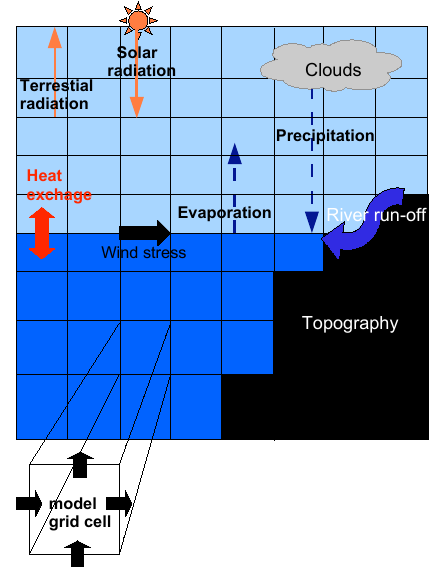
\includegraphics[scale=.4]{figs/t4inciso_1.png}
\caption{Esquema (D\"o\"os et. al., 2016)}
\label{fig:esquemacompomod}
\end{figure}

\section{Modelo de circulación atmosférica}
Las ecuaciones de conservación de momento (en las tres componentes de la velocidad),
ecuación de conservación de masa (continuidad) y energía (basado en la primera ley de la termodinámica).
Ecuación de de estado de los gases.

\section{Elípticas, parabólicas o hiperbólicas}
La ecuaciones diferenciales parciales (EDP) de segundo orden
con coeficientes constantes 
\begin{equation}
 a\ppder{u}{x} + b\ppcder{u}{x}{y} + c\ppder{u}{y} +
  d\pder{u}{x} + e\pder{u}{y} + fu + g = 0
  \label{eq:pdeg}
\end{equation}
donde ${a,b, ..., g}$ son constantes, 
se clasifican de acuerdo a los criterios de la tabla en 
la \autoref{sec:criterioclas}.

\begin{equation}
\ppder{u}{t} = c_0^2 \ppder{u}{x}
\label{eq:onda}
\end{equation}

\begin{equation}
\ppder{u}{x} + \ppder{u}{y} = 0 \; (\text{ o bien } f(x,y))
\label{eq:laplaceopoisson}
\end{equation}

\begin{equation}
\pder{T}{t} = c_0 \ppder{T}{x} \text{ donde } k>0
\label{eq:enfriamiento}
\end{equation}

\begin{equation}
\ppder{u}{x} + \ppder{u}{y} + \lambda^2 u = 0
\label{eq:Helmholtz2d}
\end{equation}

\autoref{eq:onda} $a \rightarrow 1$, $b \rightarrow 1$ y $c \rightarrow - c_0^2$

entonces $b^2 -4ac = 4 c_0^2 > 0$ $\Rightarrow$ hiperbólica

\autoref{eq:laplaceopoisson} $a \rightarrow 1$, $b \rightarrow 0$ y $c \rightarrow 1$

entonces $b^2 -4ac = -4 < 0$ $\Rightarrow$ Elíptica

\autoref{eq:enfriamiento} $u \rightarrow T$, $a \rightarrow k$, $b \rightarrow 0$ y $c \rightarrow 0$

entonces $b^2 -4ac = 0$ $\Rightarrow$ Parabólica

\autoref{eq:Helmholtz2d} $a \rightarrow 1$, $b \rightarrow 0$ y $c \rightarrow 1$

entonces $b^2 -4ac = -4 < 0$ $\Rightarrow$ Elíptica

\section{... criterio de clasificación}\label{sec:criterioclas}
\begin{center}
\begin{tabular}{lc}
\hline
	Elíptica & $b^2 - 4ac < 0$\\
	Parabólica & $b^2 - 4ac = 0$\\
	hiperbólica & $b^2 - 4ac > 0$\\
\hline
\end{tabular}
\end{center}

 Otros ejemplos de Ecuaciones Diferenciales Parciales (\ref{eq:pdeg}) son:
 \begin{equation}
	\ppder{u}{x} + \ppder{u}{y} + k(E-V)u = 0
	\label{eq:Schrodinger}
\end{equation}

 \begin{equation}
	\pder{u}{t} - \alpha\left( \ppder{u}{x} + \ppder{u}{y} + \ppder{u}{z} \right) = q
	\label{eq:heat}
\end{equation}

 \begin{equation}
	\ppder{u}{t} = v^2 \left( \ppder{u}{x} + \ppder{u}{y} \right); \; v = \sqrt{gH}
	\label{eq:propagatsunami}
\end{equation}

\begin{center}
\begin{tabular}{lc}
\hline
	Elíptica & \autoref{eq:Schrodinger} (ec de Schr\"odinger) \\
	Parabólica & \autoref{eq:heat} (ec de calor con fuente)\\
	hiperbólica & \autoref{eq:propagatsunami} (propagación tsunami)\\
\hline
\end{tabular}
\end{center}

\section{Criterio de Courant-Friedrichs-Lewy}
El criterio de Courant-Friedrichs-Lewy es una condición que debe cumplirse para que el método de diferencias finitas se mantenga estable. Restringe el tamaño del paso de tiempo y/o espacio.

Se debe cumplir
\begin{equation}
	c \leq \frac{\Delta x}{\Delta t}
	\label{eq:Courant}
\end{equation}

\newcommand\derord[3][]{
\def\temp{#1}\ifx\temp\empty
	\ensuremath {\left( \dfrac{\mathrm{d}#2}{\mathrm{d}#3}}
	\right)_j%
\else
	\ensuremath {\left(
	\dfrac{\mathrm{d}^#1#2}{\mathrm{d}#3^#1}} \right)_j%
\fi}
\newcommand\dero[2]{\ensuremath {\left( \dfrac{\mathrm{d}#1}{\mathrm{d}#2}} \right)}
\newcommand\Dt{\ensuremath {\left( \Delta t \right)}}
\newcommand\Dx{\ensuremath {\left( \Delta x \right)}}
\newcommand\dDx{\ensuremath {\left( 2\Delta x \right)}}
\newcommand\dxdero[3]{\ensuremath {\Dt^{\the\numexpr #3 - 1\relax} \derord[#3]{#1}{#2} }}

\section{Aproximación de la derivada en diferencias hacia adelante, hacia atrás y centradas}
\begin{equation}
x_{j+1} = x_j + \Dt\derord{x}{t} + \frac12\Dt^2\derord[2]{x}{t}
+ \frac1{3!}\Dt^3\derord[3]{x}{t} + \cdots
\end{equation}

\begin{equation}
\frac{x_{j+1} - x_{j}}{\Dt} =  \derord{x}{t} +
\frac12\Dt\derord[2]{x}{t} + 
	\frac1{3!}\dxdero{x}{t}{3} + \cdots
	\label{eq:forward}
\end{equation}

\begin{equation}
x_{j-1} = x_j - \Dt\derord{x}{t} + \frac12\Dt^2\derord[2]{x}{t}
- \frac1{3!}\Dt^3\derord[3]{x}{t} + \cdots
\end{equation}

\begin{equation}
\frac{x_{j-1} - x_j}{\Dt} = - \derord{x}{t} +
\frac12\Dt\derord[2]{x}{t} - 
	\frac1{3!}\dxdero{x}{t}{3} + \cdots
	\label{eq:backward}
\end{equation}

De las ecs \eqref{eq:forward} y \eqref{eq:backward} se deduce la aproximaci\'on de $\derord{x}{t}$ en diferencias hacia adelante (\autoref{eq:adelante}), diferencias hacia atrás (\autoref{eq:atras})
\begin{equation}
	\derord{x}{t} \approx \frac{x_{j+1} - x_{j}}{\Dt}
	\label{eq:adelante}
\end{equation}
\begin{equation}
	\derord{x}{t} \approx \frac{x_{j} - x_{j-1}}{\Dt}
	\label{eq:atras}
\end{equation}

y diferencias centradas (\autoref{eq:centradas})
\begin{equation}
	\derord{x}{t} \approx \frac{x_{j+1} - x_{j-1}}{2\Dt}
	\label{eq:centradas}
\end{equation}
En la \autoref{eq:centradas} significa que calculamos 
la derivada alrededor de un tiempo $j$ tomando la diferencia de los valores
correspondientes a un tiempo adelante que $j$: $j+1$ y un tiempo atrás de $j$: $j-1$ dividido por dos veces el tamaño de paso de tiempo.

\section{El esquema numérico de diferencias finitas hacia atrás es de orden 1}

%%%%%%%%
\begin{equation}
x_{j-1} = x_j - \Dt\derord{x}{t} + \frac12\Dt^2\derord[2]{x}{t}
- \frac1{3!}\Dt^3\derord[3]{x}{t} + \cdots
\end{equation}

\begin{equation}
\frac{x_{j-1} - x_j}{\Dt} = - \derord{x}{t} +
\frac12\Dt\derord[2]{x}{t} - 
	\frac1{3!}\dxdero{x}{t}{3} + \cdots
\end{equation}

\begin{equation}
\frac{x_{j} - x_{j-1}}{\Dt} = \derord{x}{t} -
\frac12\Dt\derord[2]{x}{t} + \frac1{3!}\dxdero{x}{t}{3} -
\cdots
\end{equation}

\begin{equation}
\epsilon = - \frac12\Dt\derord[2]{x}{t} + \frac1{3!}\dxdero{x}{t}{3} - \cdots
\end{equation}

\begin{equation}
\therefore \epsilon = O\Dt
\end{equation}
%%%%%%%%%

Ahora para mostrar que las diferencias centradas tienen hasta un error de orden 2,
aproximamos $u_{j+1}$ y $u_{j-1}$ expandiendo la serie de Taylor alrededor del punto $j$
% u_{j+1}
\begin{equation}
u_{j+1} = u_j + \Dx\derord{u}{x} + 
\frac12\Dx^2\derord[2]{u}{x} + 
\frac1{3!}\Dx^3\derord[3]{u}{x} + \cdots
\label{eq:ujp1}
\end{equation}

% u_{j-1}
\begin{equation}
u_{j-1} = u_j - \Dx\derord{u}{x} + 
\frac12\Dx^2\derord[2]{u}{x} - 
\frac1{3!}\Dx^3\derord[3]{u}{x} + \cdots
\label{eq:ujm1}
\end{equation}

Restamos las dos ecs y luego dividiremos por $2\Dx$ 

\eqref{eq:ujp1} - \eqref{eq:ujm1}:
\begin{equation}
u_{j+1} - u_{j-1} = 0 + 2\Dx\derord{u}{x} + 0 +
\frac2{3!}\Dx^3\derord[3]{u}{x} + 0 +
\frac2{5!}\Dx^5\derord[5]{u}{x} + \cdots
\label{eq:ujp1mujm1}
\end{equation}

\eqref{eq:ujp1mujm1} / $( 2\Dx )$:
\begin{equation}
\frac{u_{j+1} - u_{j-1}}{2\Dx} = \derord{u}{x} +
\frac1{3!}\Dx^2\derord[3]{u}{x} +
\frac1{5!}\Dx^4\derord[5]{u}{x} + \cdots
\label{eq:ujp1mujm1_s}
\end{equation}

\begin{equation}
	\therefore \epsilon = O(\Dx^2)
\end{equation}

\section{Ecuación de advección con el esquema de diferencias centradas}
\lstinputlisting[language=Matlab]{./MatlabCodes/t4inciso8.m}
%%%%%
\begin{figure}[!ht]
\centering
  \hfill\subfloat[]{
  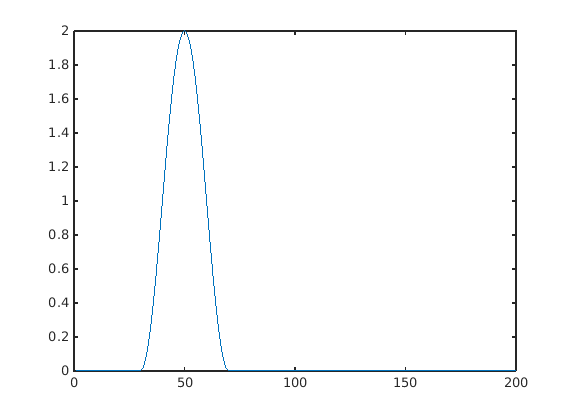
\includegraphics[width=0.35\textwidth]{t4i8_1}
  }\hfill
  \subfloat[]{%\label{fig:}
  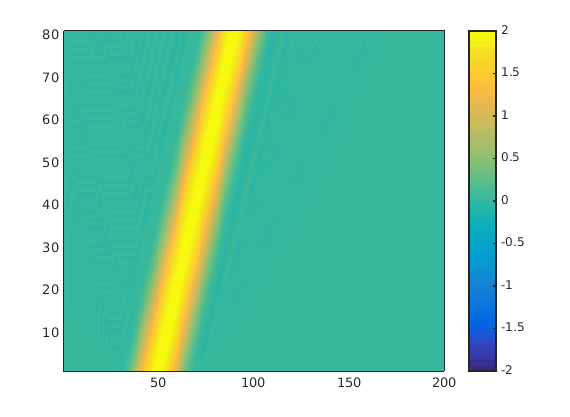
\includegraphics[width=0.35\textwidth]{t4i8_2}
  }\hfill
  \caption{a) condicion inicial y b) su evolución.}%
\label{fig:t4i8}
\end{figure}
%%%%%


\section{Esquema de salto de rana y estabilidad}
\lstinputlisting[language=Matlab]{./MatlabCodes/t4inciso9.m}
\begin{figure}[htp]
\centering
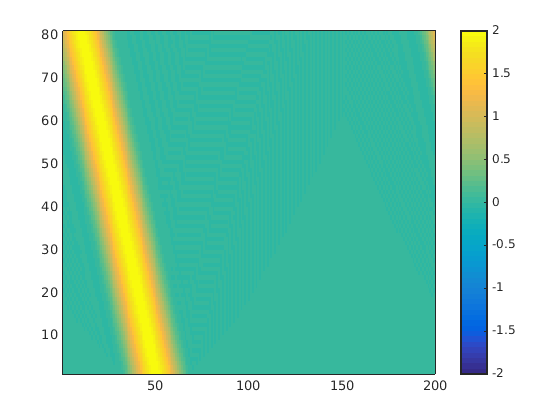
\includegraphics[scale=0.40]{figs/t4i9_2.png}
\caption{$c=-.5$}
\label{fig:t4i9}
\end{figure}
En la \autoref{fig:t4i9} se muestra el resultado de cambiar el valor de $c$ a $-.5$, 
es decir el coseno desfasado en la vertical de la condición inicial se mueve a la izquierda con el paso del tiempo.

También se encontró que la resolución temporal $\Dt$
debe ser menor a .35 cuando se fija el valor de $c=2$,
así la \autoref{eq:Courant} se sigue respetando.

\section{Esquema de diferencias centradas con \texorpdfstring{$O\left( (\Delta x)^4 \right)$}{} error de orden 4}

% u_{j+2}
\begin{equation}
u_{j+2} = u_j + \dDx\derord{u}{x} +
\frac12\dDx^2\derord[2]{u}{x} +
\frac1{3!}\dDx^3\derord[3]{u}{x} + \cdots
\label{eq:ujp2}
\end{equation}

% u_{j-2}
\begin{equation}
u_{j-2} = u_j - \dDx\derord{u}{x} +
\frac12\dDx^2\derord[2]{u}{x} -
\frac1{3!}\dDx^3\derord[3]{u}{x} + \cdots
\label{eq:ujm2}
\end{equation}

\eqref{eq:ujp2} - \eqref{eq:ujm2}:
\begin{equation}
u_{j+2} - u_{j-2} = 0 + 2\dDx\derord{u}{x} + 0 +
\frac2{3!}\dDx^3\derord[3]{u}{x} + 0 +
\frac2{5!}\dDx^5\derord[5]{u}{x} + \cdots
\label{eq:ujp2mujm2}
\end{equation}

\begin{equation}
\frac{u_{j+2} - u_{j-2}}{2\dDx} = \derord{u}{x} +
\frac1{3!}\dDx^2\derord[3]{u}{x} +
\frac1{5!}\dDx^4\derord[5]{u}{x} + \cdots
\label{eq:ujp2mujm2_s}
\end{equation}

El objetivo es eliminar el término con orden cuadrático
$\dDx^2\derord[3]{u}{x}$, 
necesitamos los coeficientes apropiados $\frac43$ y $\frac13$


\begin{equation}
\def\coef{\frac43}
\coef\frac{u_{j+1} - u_{j-1}}{2\Dx} = \coef\derord{u}{x} +
\coef\frac1{3!}\Dx^2\derord[3]{u}{x} +
\coef\frac1{5!}\Dx^4\derord[5]{u}{x} + \cdots
\label{eq:4tercios}
\end{equation}

\begin{equation}
\def\coef{\frac13}
\coef\frac{u_{j+2} - u_{j-2}}{2\dDx} = \coef\derord{u}{x} +
\coef\frac1{3!}\dDx^2\derord[3]{u}{x} +
\coef\frac1{5!}\dDx^4\derord[5]{u}{x} + \cdots
\label{eq:1tercio}
\end{equation}

Hacemos $(4/3)$\eqref{eq:ujp1mujm1_s} -
$(1/3)$\eqref{eq:ujp2mujm2_s} =
\eqref{eq:4tercios} - \eqref{eq:1tercio}:
\begin{equation}
\def\u{\frac13}
\def\c{\frac43}
    \begin{split}
\c\frac{u_{j+1} - u_{j-1}}{2\Dx}-\u\frac{u_{j+2} -
u_{j-2}}{2\dDx} = & \derord{u}{x} + \cancel{ \left[
\c\frac{1}{3!} - \u\frac{1}{3!}(2)^2 \right] }
\Dx^2\derord[3]{u}{x} + \\
& \left[ \c\frac{\Dx^4}{5!} - \u\frac{\dDx^4}{5!}
\right]\derord[5]{u}{x} + \\
& \left[ \c\frac{\Dx^6}{7!} - \u\frac{\dDx^6}{7!}
\right]\derord[7]{u}{x} + \cdots
    \end{split}
\label{eq:o4}
\end{equation}

\begin{equation}
\def\u{\frac13}
\def\c{\frac43}
    \begin{split}
\c\frac{u_{j+1} - u_{j-1}}{2\Dx}-\u\frac{u_{j+2} -
u_{j-2}}{2\dDx} = & \derord{u}{x} + 
\left[ -\frac{1}{30} \right]\Dx^4\derord[5]{u}{x} + \\
& \left[ -\frac{1}{252} \right]\Dx^6\derord[7]{u}{x} + \cdots
    \end{split}
\label{eq:o4_s}
\end{equation}

\begin{equation}
	\therefore \epsilon = O\left( \Dx^4 \right)
\end{equation}

\end{document}